\documentclass[12pt]{article}
\usepackage[utf8]{inputenc}
\usepackage[margin=1in]{geometry}
\usepackage[spanish]{babel}\decimalpoint
\usepackage{setspace}\onehalfspacing
\usepackage{parskip} % Espacio entre parrafos.
\usepackage{graphicx} % Para usar comando \includegraphics[]{}
\usepackage{amssymb} % Para usar el simbolo del conj. de los Reales.
\usepackage{amsmath} % Para usar columnas vectoriales.
\usepackage{multirow} % Para unir multiples filas en una tabla.
\usepackage{hyperref} % Siempre debe ser el ultimo paquete.


\setcounter{tocdepth}{2} % Que no incluya subsubsections en la tabla de contenidos (toc).

%================================

\title{Clase 22. Aplicación de las Integrales: Volúmenes a partir de Rebanadas.}
\author{MIT 18.01: Single Variable Calculus.}
\date{}


\begin{document}

\maketitle

\begin{abstract}
\noindent Las integrales también pueden ser usadas para calcular el volumen de una figura. El procedimiento es similar al usado en las áreas de la clase anterior: debemos buscar el integrando y los límites de la integral, para después aplicar el TFC 1. Para ello, revisaremos dos métodos: \textbf{de los discos} y \textbf{del caparazón}.
\end{abstract}


\section{Aproximando al volumen de un sólido cilíndrico.}

Una forma de conocer el volumen de un sólido (i.e, una figura de tres dimensiones), es cortándolo en $n$ \textbf{rebanadas}, aproximar sus volúmenes al de un \textbf{sólido cilíndrico} y sumarlos por medio de una integral.

Un sólido cilíndrico es una figura que consiste de dos regiones planas congruentes (o caras), que son unidas por segmentos perpendiculares a ellas.


El volumen $V$ de un sólido cilíndrico se calcula como el producto entre el área $A$ de su base (es decir, de una de sus caras) y su altura $h$, que es dada por la distancia de los segmentos que unen sus caras. 
\[
  V = Ah
\]

\begin{figure}[hbt!]
\centering
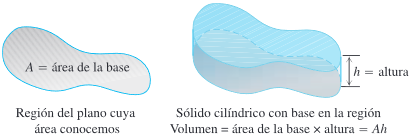
\includegraphics[scale=0.6]{img/solid-cylindric.jpg}
\caption{Fuente: (Thomas, 2010: 308).}
\end{figure}

\newpage

En ese sentido, si tenemos un sólido cilíndrico de base circular (el que quizá más conocemos), su volumen será $V = (\pi \cdot  r^{2}) \cdot h$. Mientras que si es rectangular\footnote{También conocido como caja rectangular o paralelepipedo rectangular.}, $V = (l \cdot w) \cdot h$, con $l =$ largo y $w =$ ancho.

\begin{figure}[hbt!]
\centering
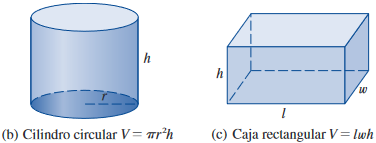
\includegraphics[scale=0.6]{img/solid-cylindric-examples.jpg}
\caption{Fuente: (Stewart, 2017: 438).}
\end{figure}

La idea es usar este volumen $V = Ah$ para aproximarnos al de un sólido que es irregular.

Por ejemplo, supongamos que queremos calcular el volumen de un sólido como el que vemos a continuación. Lo que haremos primero, es cortar una rebanada\footnote{Más específicamente, son dos secciones transversales (\textit{cross-sectional}) que unidas forman la rebanada.} perpendicular al eje $x$ y luego calcularemos su volumen.

\begin{figure}[hbt]
\centering
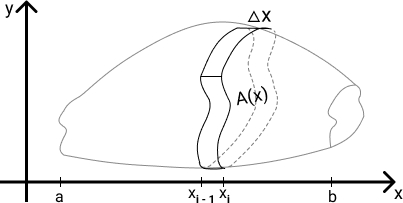
\includegraphics[scale=0.55]{img/solido-clases.jpg}
\end{figure}

Si nos damos cuenta, la rebanada es similar a un sólido cilíndrico: tiene dos caras que son congruentes y se unen horizontalmente por segmentos que acá son curvados y no rectos. Por lo tanto, \textbf{el volumen de esta rebanada lo aproximaremos al del sólido cilíndrico}.

La altura de la rebanada corresponde a su ancho calculado como $\Delta x = x_{i} - x_{i - 1}$; mientras que el área de su base\footnote{Es decir, el área de una sección transversal.} será $A(x)$, porque dependerá del lugar en $x$ donde realicemos el corte. De este modo, el volumen de esta $i$-ésima rebanada $V_{i}$ lo calculamos como:
\[
  V_{i} \approx A(x) \Delta x
\]
Nuestra idea es cortar $n$ rebanadas de igual ancho (i.e, $\Delta x = (x_{i} - x_{i - 1})/n$) al sólido, calcular sus volúmenes como la aproximación de arriba y sumarlos, cuyo valor denotaremos como $V$:
\[
  V \approx \sum_{i = 1}^{n} A(x_{i}) \Delta x
\]
Como vemos, aún seguirá siendo una aproximación. Para precisar este volumen, calcularemos su límite a medida que $n \to \infty$, obteniendo la integral de este sólido, cuyo volumen está entre $x = a$ y $x = b$.
\[
  V = \lim_{n \to \infty} \left(\sum_{i = 1}^{n} A(x_{i}) \Delta x\right) = \int_{a}^{b} A(x)dx
\]
La integral $V$ también podemos verla de la siguiente manera. Debido a que $A(x)$ va cambiando según dónde realicemos el corte y que $\Delta x$ también lo hará dependiendo de la cantidad $n$ de rebanadas que generemos, el cambio en el volumen de una de ellas será:
\[
  \Delta V_{i} \approx A(x) \Delta x
\]
Si dichas rebanadas las cortamos infinitamente delgadas o, a medida que $\Delta x \to 0$, entonces:
\[
  dV_{i} = A(x) dx
\]
Con $dV_{i}$ podemos hacer seguimiento del cambio infinitesimal del volumen de cada rebanada. Si las sumamos, obtenemos el volumen $V$ como una integral definida en $a \leq x \leq b$.
\[
  V = \int_{a}^{b} dV = \int_{a}^{b} A(x)dx
\]


\section{Sólidos de Revolución.}

Un \textbf{Sólido de Revolución} es aquel que se genera al hacer girar una figura plana alrededor de una recta horizontal o verticalmente. Su volumen se calcula aproximándolo al de un sólido cilíndrico y, en esta ocasión, veremos dos métodos: el de Los Discos y el del Caparazón Cilíndrico.

\subsection{Método de los Discos.}

Un método para calcular el volumen de un sólido de revolución, es el \textbf{de Los Discos}. Consiste en dividir el área bajo la curva de una función en \textbf{rectángulos verticales a una recta horizontal y hacerlos girar alrededor de ella}, generándose discos con ellos.

\begin{figure}[hbt!]
\centering
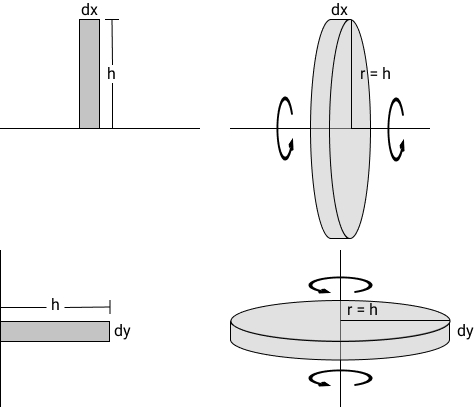
\includegraphics[scale=0.5]{img/disk-method-3.jpg}
\end{figure}

En ese sentido, la suma de los volúmenes de los discos será igual al del sólido de revolución.

El disco es un sólido cilíndrico, así que su volumen podemos calcularlo como $V_{i} \approx A(x) \Delta x$, donde $A(x)$ es el área de su sección transversal, que es un \textbf{círculo} de radio $r$ igual a la altura $h$ del rectángulo. Por lo tanto, $V_{i} \approx (\pi r^{2}) \Delta x$ y la suma de cada $V_{i}$ cuando $n \to \infty$ es:
\[
  V = \int_{a}^{b} (\pi r^{2}) dx \quad \text{o} \quad V = \int_{a}^{b} (\pi r^{2}) dy
\]
\textbf{Ejemplo 1.} \quad Calcule el volumen de la siguiente esfera de radio $r = a$.

\begin{figure}[hbt!]
\centering
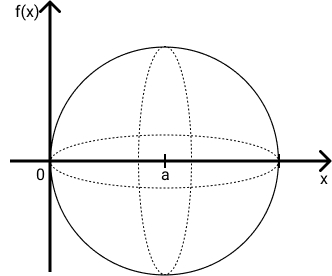
\includegraphics[scale=0.5]{img/sphere-example-1.jpg}
\end{figure}

\textbf{Solución.} \quad Para resolver este ejercicio, usaremos el método de los discos con respecto a $x$. Lo primero será cortar la mitad de una sección transversal de la esfera, que equivale a un semicírculo y dividamos su área con un rectángulo vertical.

\newpage

\begin{figure}[hbt!]
\centering
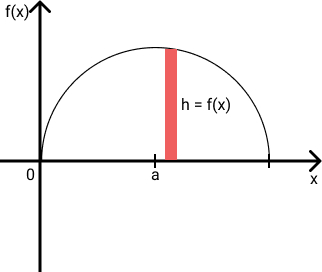
\includegraphics[scale=0.5]{img/sphere-example-3.jpg}
\end{figure}

Veamos que la altura del rectángulo varía con respecto a $x$ o, en otras palabras, $h = f(x) - 0 = f(x)$. Por lo tanto, debemos buscar esta función.

Como la sección transversal de la esfera es un círculo, podemos usar la ecuación del círculo para encontrar la función del semicírculo. Su radio es $r = a$ y su centro está en $C(a, \ 0)$.
\begin{align*}
(x - a)^{2} + (f(x) - 0)^{2} &= a^{2} \\
f(x) &= \pm \sqrt{2ax - x^{2}}
\end{align*}
Como estamos trabajando con el semicírculo superior, usaremos $f(x) = \sqrt{2ax - x^{2}}$.

Para calcular el volumen de la esfera, debemos saber dónde delimita con respecto a $x$. Veamos que parte en $x = 0$ y termina en el valor de su diámetro $d = 2r = 2a$. En consecuencia:
\[
  V = \int_{0}^{2a} \left[\pi \cdot \left(\sqrt{2ax - x^{2}}\right)^{2} \right] dx
    = \pi \left[2a\left(\frac{x^{2}}{2}\right) - \frac{x^{3}}{3}\right]_{0}^{2a}
    = \frac{4}{3} \pi a^{3}
\]

\subsection{Método del Caparazón Cilíndrico.}

El volumen de un sólido de revolución también podemos obtenerlo con el \textbf{método del caparazón cilíndrico}. En éste también se divide el área de una figura plana en rectángulos verticales a una recta horizontal, pero se hacen girar de forma paralela a dicha línea, lo que produce cilindros abiertos con un borde grueso a lo largo de la superficie.

\newpage

\begin{figure}[hbt!]
\centering
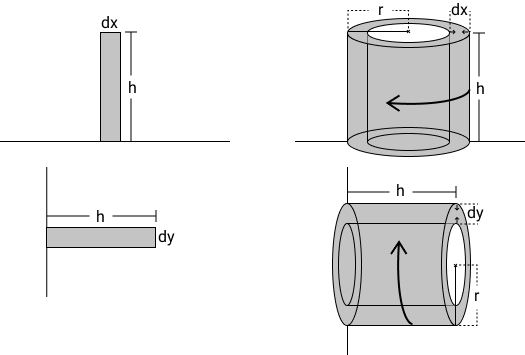
\includegraphics[scale=0.6]{img/shell-method-4.jpg}
\end{figure}

La idea es aproximarnos al volumen del sólido de revolución a partir del caparazón. Como es un sólido cilíndrico, corresponde a $V_{i} \approx A(x) \Delta x$. Su sección transversal la obtenemos al abrirlo a lo largo de éste que, como vemos a continuación, es un paralelepipedo rectangular.

\begin{figure}[hbt!]
\centering
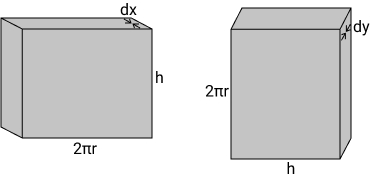
\includegraphics[scale=0.6]{img/shell-method-5.jpg}
\end{figure}

Observemos, también, que el largo del paralelepipedo es la circunferencia de la sección transversal circular del caparazón cilíndrico. Por lo tanto, el área de este último es $A(x) = (2 \pi r) \cdot h$ y su volumen:
\[
  V_{i} \approx [(2 \pi r) \cdot h] \Delta x
\]
En consecuencia, el volumen del sólido de revolución será la suma de los $V_{i}$ a medida que $n \to \infty$:
\[
  V = \int_{a}^{b} [(2 \pi r) \cdot h] dx \quad \text{o} \quad V = \int_{a}^{b} [(2 \pi r) \cdot h] dy
\]
\textbf{Ejercicio 2.} \quad Calcule el volumen de la caldera usando el método del caparazón.

\newpage

\begin{figure}[hbt!]
\centering
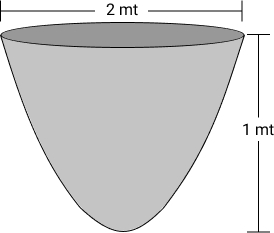
\includegraphics[scale=0.5]{img/cauldron-example-1.jpg}
\end{figure}

\textbf{Solución.} \quad La caldera podemos modelarla como el sólido de revolución de $f(x) = x^{2}$, manteniendo sus medidas de alto y largo.

\begin{figure}[hbt!]
\centering
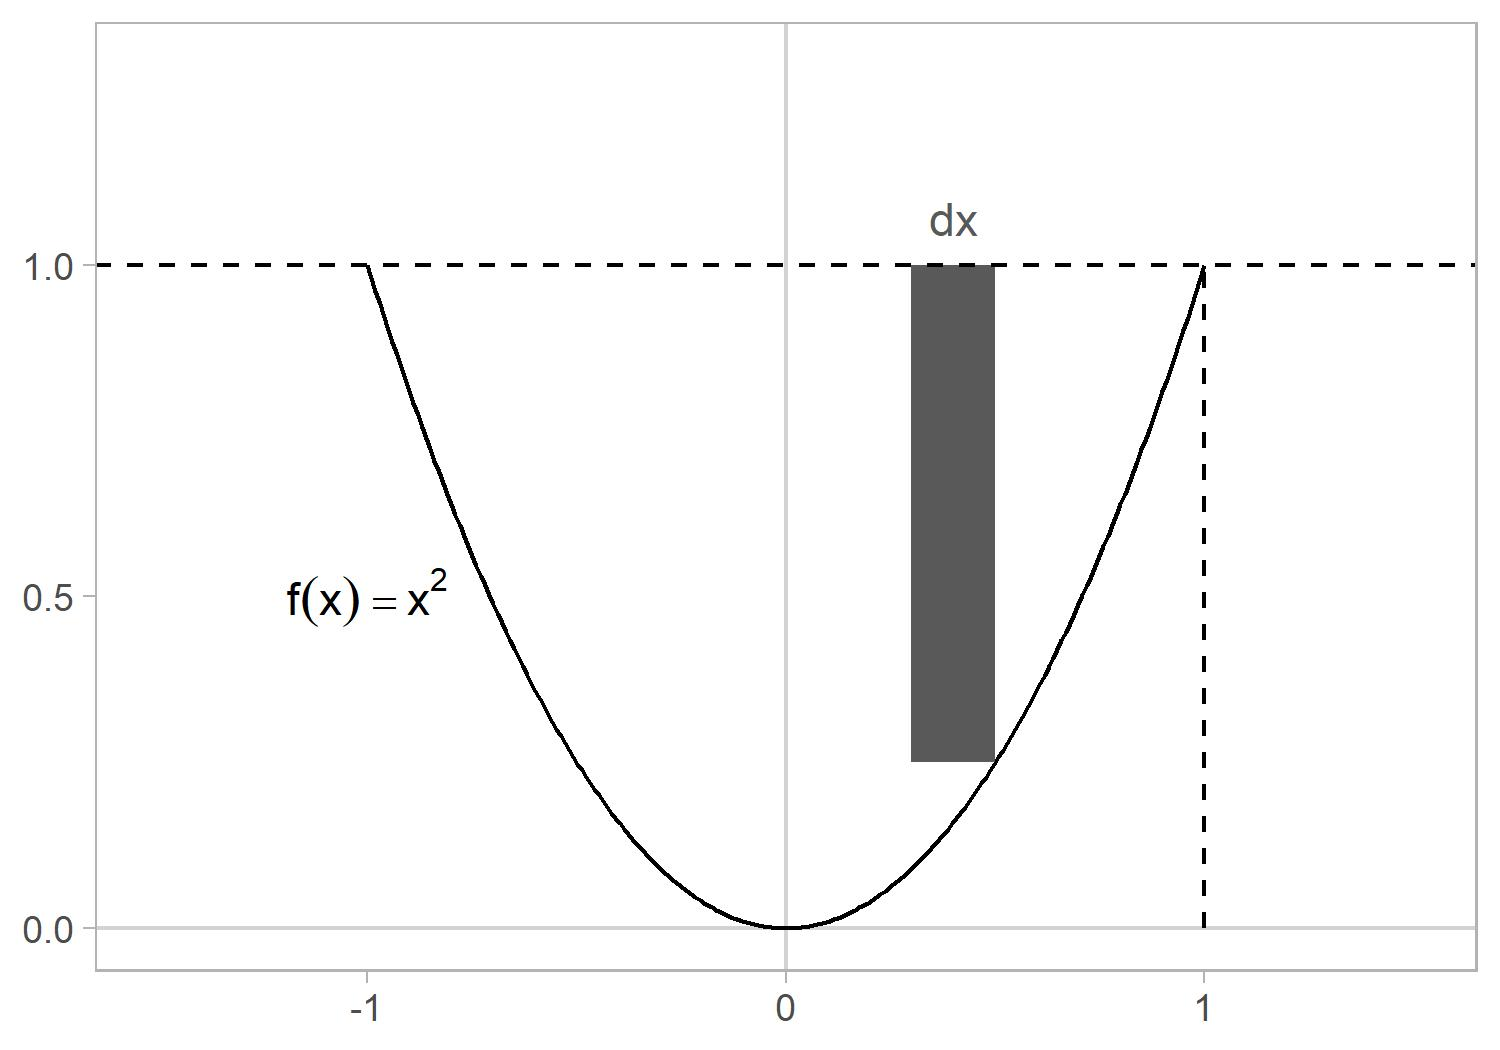
\includegraphics[scale=0.7]{img/cauldron-example-2.jpg}
\end{figure}

Para generar el sólido, solo necesitamos una de las dos mitades de la parábola. En este caso, trabajaremos entre $0 \leq x \leq 1$.

Como nos piden usar el método del caparazón para calcular el volumen de la caldera, necesitamos conocer el valor del radio $r$ y la altura $h$ del sólido cilíndrico. En el gráfico de la parábola se puede apreciar a partir del rectángulo, que ambas medidas varían con respecto al valor de $x$ en el intervalo $[0, \ 1]$. Es decir:
\[
  r = x - 0 = x \qquad \qquad h = 1 - x^{2}
\]
Por lo tanto, el volumen $V$ de la caldera a partir del método del caparazón y con respecto a $x$, corresponde a:
\[
  V = \int_{0}^{1} [(2 \pi x) (\text{m}) \cdot (1 - x^{2}) (\text{m})]dx (\text{m})
    = 2 \pi \left[\frac{x^{2}}{2} - \frac{x^{4}}{4}\right]_{0}^{1}
    = \frac{\pi}{2} \text{ m}^{3}
    \approx 1571 \text{ Lt}
\]
Generalicemos el volumen de la caldera. Digamos que su altura es $a$, un valor sin unidades de medida. Por tanto, su ancho será de $\sqrt{a} - (-\sqrt{a}) = 2\sqrt{a}$ y la altura del caparazón cilíndrico $h = a - x^{2}$. En consecuencia:
\[
V = \int_{0}^{\sqrt{a}} [(2 \pi x) \cdot (a - x^{2})]dx
  = 2 \pi \cdot \left[\frac{ax^{2}}{2} - \frac{x^{4}}{4}\right]_{0}^{\sqrt{a}}
  = \frac{\pi}{2} a^{2}
\]
La próxima clase usaremos la misma caldera, pero la llenaremos de agua y calcularemos el calor necesario para hervirla (i.e, que alcance su punto de ebullición de $100^{\circ}$C), considerando que afuera de ella hay $0^{\circ}$C.

Veremos que la temperatura del agua variará con respecto a la altura de la caldera. Por lo tanto, vamos a obtener la energía necesaria para hervirla como la suma de la temperatura de cada volumen infinitamente delgado de este contenedor.

\end{document}
